\documentclass[tikz,border=10pt]{standalone}
\usetikzlibrary{arrows.meta, positioning, calc, decorations.pathreplacing}
\usepackage{amssymb}

\begin{document}
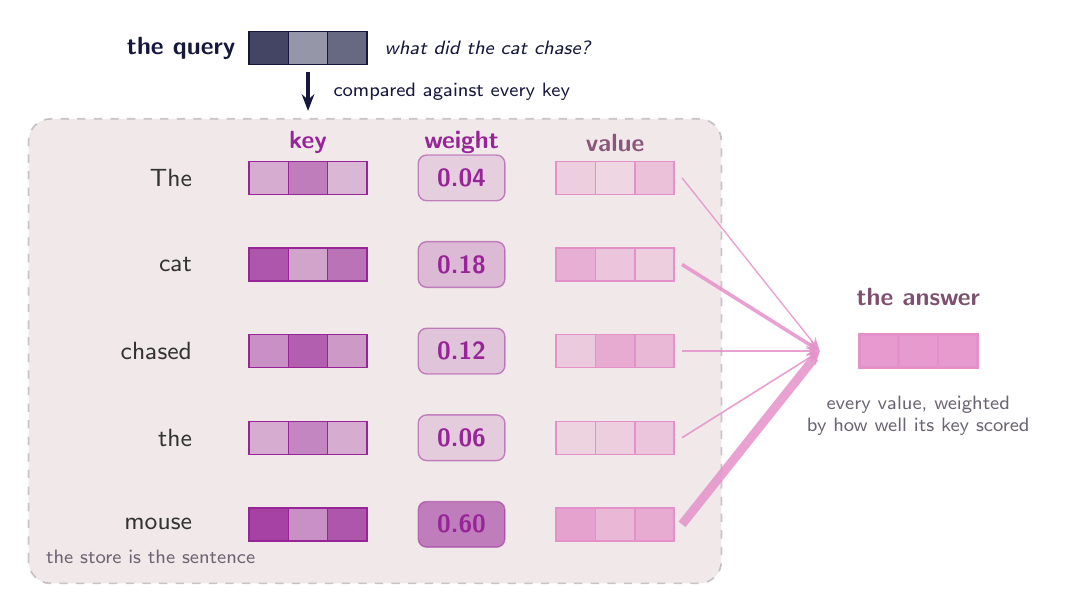
\begin{tikzpicture}[
    every node/.style={font=\sffamily},
]

% ---------------------------------------------------------------- colours
\definecolor{c1}{HTML}{15173D}   % QUERY
\definecolor{c2}{HTML}{982598}   % KEYS, and the weights they produce
\definecolor{c3}{HTML}{E491C9}   % VALUES, and the blended answer
\definecolor{c4}{HTML}{F1E9E9}   % the store panel
\definecolor{axiscolor}{HTML}{333333}
\definecolor{labelcolor}{HTML}{6B6472}

\tikzset{
    word/.style={font=\sffamily\small, text=axiscolor, anchor=east},
    kcell/.style={rectangle, minimum width=0.5cm, minimum height=0.42cm,
                  draw=c2, line width=0.5pt, fill=c2},
    vcell/.style={rectangle, minimum width=0.5cm, minimum height=0.42cm,
                  draw=c3, line width=0.5pt, fill=c3},
    qcell/.style={rectangle, minimum width=0.5cm, minimum height=0.42cm,
                  draw=c1, line width=0.5pt, fill=c1},
    ocell/.style={rectangle, minimum width=0.5cm, minimum height=0.42cm,
                  draw=c3, line width=1.0pt, fill=c3, fill opacity=0.92},
}

% ================================================================
% GEOMETRY
%   rows (one per word)  y = 5.7, 4.6, 3.5, 2.4, 1.3
%   word label           x = 0.75 (anchor east)
%   key vector           x = 1.35 .. 2.85
%   weight               x = 4.05
%   value vector         x = 5.25 .. 6.75
%   blended answer       x = 8.85 .. 10.35, y = 3.5
%   the query            y = 7.35, above the key column
% ================================================================

% ---------------------------------------------------------------- the store
\fill[c4, rounded corners=8pt] (-1.45, 0.55) rectangle (7.35, 6.45);
\draw[labelcolor, opacity=0.35, dashed, line width=0.6pt, rounded corners=8pt]
    (-1.45, 0.55) rectangle (7.35, 6.45);
\node[font=\sffamily\scriptsize, text=labelcolor, anchor=south west]
    at (-1.35, 0.68) {the store is the sentence};

% ---------------------------------------------------------------- headers
\node[font=\sffamily\small\bfseries, text=c2] at (2.1, 6.15) {key};
\node[font=\sffamily\small\bfseries, text=c2] at (4.05, 6.15) {weight};
\node[font=\sffamily\small\bfseries, text=c3!60!black] at (6.0, 6.15) {value};

% ---------------------------------------------------------------- rows
% word / y / key cell opacities / weight / value cell opacities / arrow width
\foreach \w/\y/\ka/\kb/\kc/\a/\va/\vb/\vc/\aw in {%
    The/5.7/0.30/0.55/0.25/0.04/0.30/0.20/0.45/0.5,
    cat/4.6/0.75/0.35/0.60/0.18/0.65/0.40/0.30/1.3,
    chased/3.5/0.45/0.70/0.40/0.12/0.35/0.70/0.55/0.95,
    the/2.4/0.30/0.50/0.30/0.06/0.25/0.30/0.40/0.6,
    mouse/1.3/0.85/0.45/0.75/0.60/0.80/0.55/0.70/3.2%
} {
    \node[word] at (0.75, \y) {\w};

    % key vector
    \node[kcell, fill opacity=\ka] at (1.6,  \y) {};
    \node[kcell, fill opacity=\kb] at (2.1,  \y) {};
    \node[kcell, fill opacity=\kc] at (2.6,  \y) {};

    % the weight this key earns
    \fill[c2, opacity={0.10 + 0.75*\a}, rounded corners=3pt]
        (3.5, \y-0.29) rectangle (4.6, \y+0.29);
    \draw[c2, opacity=0.5, rounded corners=3pt, line width=0.5pt]
        (3.5, \y-0.29) rectangle (4.6, \y+0.29);
    \node[font=\sffamily\small\bfseries, text=c2] at (4.05, \y) {\a};

    % value vector
    \node[vcell, fill opacity=\va] at (5.5,  \y) {};
    \node[vcell, fill opacity=\vb] at (6.0,  \y) {};
    \node[vcell, fill opacity=\vc] at (6.5,  \y) {};

    % this value's share of the answer
    \draw[-{Stealth[length=5pt]}, line width=\aw pt, c3, opacity=0.85]
        (6.85, \y) -- (8.6, 3.5);
}

% ---------------------------------------------------------------- the query
\node[qcell, fill opacity=0.80] at (1.6, 7.35) {};
\node[qcell, fill opacity=0.45] at (2.1, 7.35) {};
\node[qcell, fill opacity=0.65] at (2.6, 7.35) {};
\node[font=\sffamily\small\bfseries, text=c1, anchor=east] at (1.3, 7.35)
    {the query};
\node[font=\sffamily\scriptsize, text=c1, anchor=west, align=left]
    at (2.95, 7.35) {\emph{what did the cat chase?}};

\draw[-{Stealth[length=6pt]}, line width=1.2pt, c1]
    (2.1, 7.05) -- (2.1, 6.55);
\node[font=\sffamily\scriptsize, text=c1, anchor=west] at (2.3, 6.8)
    {compared against every key};

% ---------------------------------------------------------------- the answer
\node[ocell] at (9.35, 3.5) {};
\node[ocell] at (9.85, 3.5) {};
\node[ocell] at (10.35, 3.5) {};
\node[font=\sffamily\small\bfseries, text=c3!55!black, anchor=south]
    at (9.85, 3.95) {the answer};
\node[font=\sffamily\scriptsize, text=labelcolor, anchor=north, align=center]
    at (9.85, 3.05) {every value, weighted\\by how well its key scored};

\end{tikzpicture}
\end{document}
